\documentclass[compress]{beamer}        % [compress] (written before {beamer} <=> navigation bar one line, all subsections in 1 line instead of 2

% Setup appearance:
\usetheme{CambridgeUS}
%	AnnArbor | Antibes | Bergen |
%	Berkeley | Berlin | Boadilla |
%	boxes | CambridgeUS | Copenhagen |
%	Darmstadt | default | Dresden |
%	Frankfurt | Goettingen |Hannover |
%	Ilmenau | JuanLesPins | Luebeck |
%	Madrid | Malmoe | Marburg |
%	Montpellier | PaloAlto | Pittsburgh |
%	Rochester | Singapore | Szeged |
%	Warsaw
%

\useoutertheme[footline=authorinstitute,subsection=false]{miniframes}
\usecolortheme{whale}

%	albatross | beaver | beetle |
%	crane | default | dolphin |
%	dove | fly | lily | orchid |
%	rose |seagull | seahorse |
%	sidebartab | structure |
%	whale | wolverine


\setbeamertemplate{footline}
{
  \hbox{%
  \begin{beamercolorbox}[wd=.25\paperwidth,ht=2.25ex,dp=1ex,center]{title in head/foot}%
    \usebeamerfont{date in head/foot}\insertshortauthor
  \end{beamercolorbox}%
  \begin{beamercolorbox}[wd=.5\paperwidth,ht=2.25ex,dp=1ex,center]{date in head/foot}%
    \usebeamerfont{title in head/foot}\insertshortinstitute
  \end{beamercolorbox}%
  \begin{beamercolorbox}[wd=.25\paperwidth,ht=2.25ex,dp=1ex,center]{title in head/foot}%
    \usebeamerfont{date in head/foot}
    \insertframenumber{} / \inserttotalframenumber
    %\insertframenumber{} / \insertpresentationendpage
  \end{beamercolorbox}}%
  \vskip0pt%
}

%\setbeamercolor{titlelike}{parent=structure}
%\setbeamercolor{structure}{fg=beamer@blendedblue}
%% \useinnertheme{rounded}
%\setbeamerfont{block title}{size={}}
%\usefonttheme[onlylarge]{structurebold}   % title and words in the table of contents bold
%\setbeamerfont*{frametitle}{size=\normalsize,series=\bfseries}
\setbeamertemplate{navigation symbols}{}
\setbeamercolor{frametitle}{parent=boxes, bg=white}
{ % only on titlepage


\usepackage{times}
\usepackage{amsmath,amssymb,amsthm}
\usepackage{color}
\usepackage{changepage}
\usepackage{multirow}
\usepackage[absolute,overlay]{textpos}
\usepackage{enumerate}
%\usepackage{pgfpages}
\usepackage[all]{xy}
\usepackage{textcomp}
\usepackage{etex}
\usepackage{tikz}
\usetikzlibrary{shapes}
%\usepackage{handoutWithNotes}
%\pgfpagesuselayout{4 on 1}[border shrink=1mm]




\definecolor{camblue}{RGB}{26,26,89}
\definecolor{Rblue}{RGB}{0,255,255}
\definecolor{Rdarkblue}{RGB}{0,0,255}
\definecolor{Rgreen}{RGB}{0,205,0}
\definecolor{green2}{RGB}{51,204,51}
\newcommand{\tcb}{\textcolor{beamer@blendedblue}}
\newcommand{\tcbb}{\textcolor{camblue}}
\newcommand{\tcr}{\textcolor{red}}
\newcommand{\tcg}{\textcolor{gray}}
\newcommand{\tcgr}{\textcolor{green2}}
\newcommand{\tcblk}{\textcolor{black}}
\newcommand{\tcRg}{\textcolor{Rgreen}}
\newcommand{\tcRdb}{\textcolor{Rdarkblue}}
\newcommand{\tcRb}{\textcolor{Rblue}}
\newcommand{\tcw}{\textcolor{white}}
\newcommand{\m}{\phantom{-}}
\newcommand{\bp}{\tcbb{$\bullet$}\:}


\title{{\huge Statistics for Computing\\[0.1cm]MA4413}}
\author[Kevin Burke]{{\bf\\[0.5cm]{\huge Lecture 10}\\[0.2cm]\emph{The Normal Distribution}\\[1.4cm]Kevin Burke}\\[0.3cm]\tcb{kevin.burke@ul.ie}}

\institute[University of Limerick, Maths \& Stats Dept]{}
\date{}

%\TPGrid[5mm,5mm]{1}{1}

\begin{document}


\begin{frame}[t]
\titlepage
\end{frame}


\section{Distributions}
\subsection{Distributions Studied So Far}
\begin{frame}{\bf \tcb{Distributions Studied So Far}}
\begin{itemize}\itemsep0.5cm
\item Bernoulli$(p)$
\begin{itemize}\itemsep0.1cm
\item An experiment where an event can occur with probability $p$.
\item $x \in \{0, 1\}$ $\Rightarrow$ binary variable.
\end{itemize}
\item Binomial$(n,p)$
\begin{itemize}\itemsep0.1cm
\item The number of events in $n$ Bernoulli trials.
\item $x \in \{0, 1, 2, \ldots, n\}$ $\Rightarrow$ discrete variable.
\end{itemize}
\item Poisson$(\lambda)$
\begin{itemize}\itemsep0.1cm
\item The number of events in an interval of time / distance / space.
\item $x \in \{0, 1, 2, \ldots, \infty\}$ $\Rightarrow$ discrete variable.
\end{itemize}
\item Exponential$(\lambda)$
\begin{itemize}\itemsep0.1cm
\item The time / distance / space between Poisson events occurring.
\item $t \in [0, \infty)$ $\Rightarrow$ positive continuous variable.
\end{itemize}
\end{itemize}
\end{frame}





\section{Normal Distribution}

\subsection{Normal Distribution}
\begin{frame}{\bf \tcb{Normal Distribution}\\[-1.1cm]}

\begin{center}
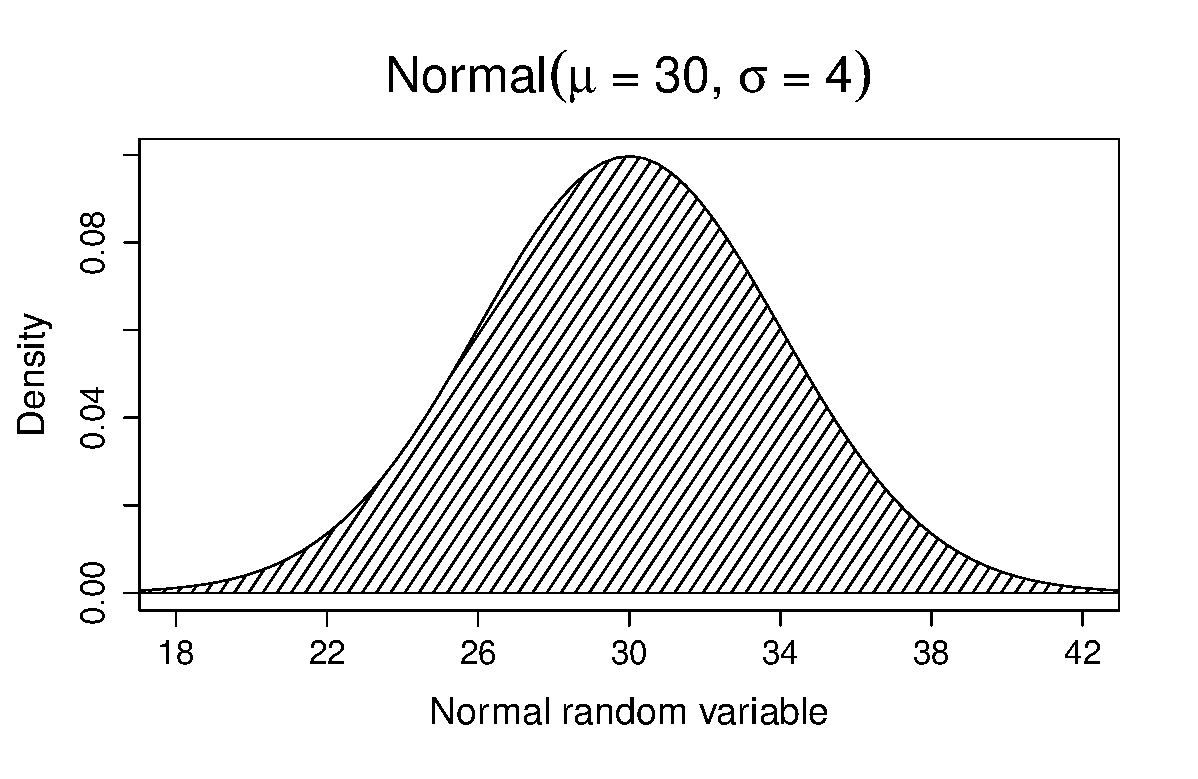
\includegraphics[width=0.87\textwidth, trim = 0.0cm 0.5cm 0.3cm 0.5cm, clip]{Normal}
\end{center}

A \emph{continuous} distribution where the probability is distributed symmetrically around a central value, i.e., the mean.

\end{frame}



\subsection{Importance of the Normal Distribution}
\begin{frame}{\bf \tcb{Importance of the Normal Distribution}}
\begin{itemize}\itemsep0.6cm
\item Many biological, geographical, economic and demographic quantities are approximately normally distributed. Hence, it is a ``normal'' distribution, i.e., typical / common in practice.
    %(note: often the $\log$ of the variable is used).
\item The mean of a \emph{sample} of data is approximately normally distributed. This is known as the \emph{central limit theorem} which underpins the most commonly used statistical testing procedures.
\item Features of mass-produced products (e.g., dimensions, weight, volume etc.) are often normally distributed which is the basis of \emph{quality control} procedures.
%\item Measurement errors are often assumed to be normally distributed.
\item Both the binomial (when $n$ is large) and Poisson distributions (when $\lambda$ is large) are approximately normal.
\end{itemize}


\end{frame}






\subsection{Normal Distribution}
\begin{frame}{\bf \tcb{Normal Distribution}}
The {\bf normal distribution} is used for \emph{continuous} variables which are distributed symmetrically around the mean value.
\begin{align*}
\boxed{X \sim \text{Normal}(\mu, \sigma)}
\end{align*}
\begin{align*}
\boxed{\Pr(X > x) = \int_x^\infty \frac{1}{\sigma \sqrt{2\,\pi}} e^{-\frac{1}{2}\left(\frac{x-\mu}{\sigma}\right)^2}\,dx}\\[-1cm]
\end{align*}
\begin{align*}
\text{where } \boxed{x \in (-\infty,\infty)}
\end{align*}
\begin{align*}
\boxed{E(X) = \mu}
\end{align*}
\begin{align*}
\boxed{Var(X) = \sigma^2}\\[-0.5cm]
\end{align*}

\end{frame}


\subsection{Normal Distribution}
\begin{frame}{\bf \tcb{Normal Distribution}}

Clearly $\mu$ is the {\bf mean} and $\sigma$ is the {\bf standard deviation} for a normally distributed random variable.\\[0.7cm]

Although $x \in (-\infty, \infty)$ \emph{in theory}, 99.7\% of the probability is distributed to $x \in [\mu - 3\,\sigma,\mu + 3\,\sigma]$, i.e., $\Pr(\mu - 3\,\sigma < X < \mu + 3\,\sigma) = 0.997.$\\[0.7cm]

Normal random variables are \emph{continuous}. Thus, we calculate \emph{greater than probabilities} (unlike the discrete cases). This is done via:\\[-0.3cm]
\begin{align*}
\Pr(X > x) = \int_x^\infty \frac{1}{\sigma \sqrt{2\,\pi}} e^{-\frac{1}{2}\left(\frac{x-\mu}{\sigma}\right)^2}\,dx.\\[-0.4cm]
\end{align*}
The above integral \emph{cannot be done by hand}. We must use statistical tables or software.


\end{frame}










\subsection{Approximating Normal Probabilities}
\begin{frame}{\bf \tcb{Approximating Normal Probabilities\\[-1.2cm]}}
\begin{center}
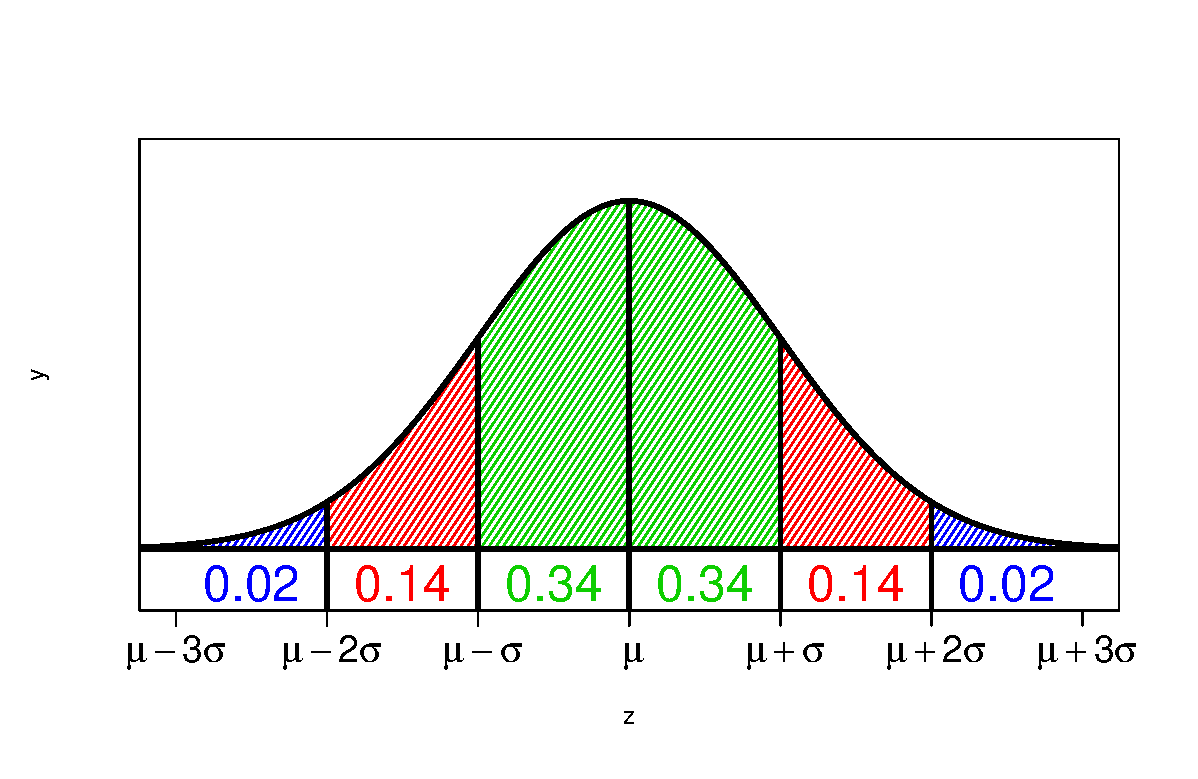
\includegraphics[width=0.98\textwidth, trim = 1.5cm 1.5cm 0.7cm 1.5cm, clip]{NormalProbs}
\end{center}
\begin{itemize}
\item The above {\bf approximate} probabilities can be used when we do not have stats tables.
\end{itemize}

\end{frame}




\subsection{Example: Salary}
\begin{frame}{\bf \tcb{Example: Salary}}
Let $X$ be the salary (in thousands) for a particular type of job where $X \sim \text{Normal}(\mu=30,\sigma=4)$. Thus we know that:

\begin{center}
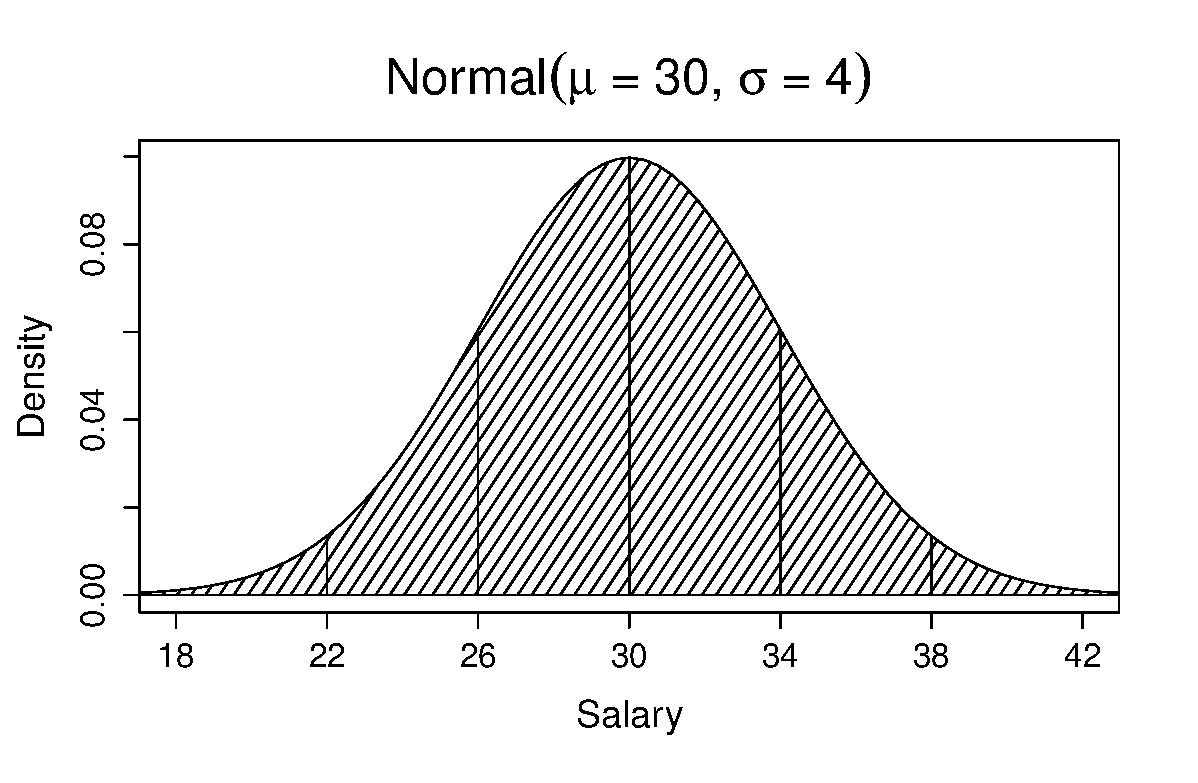
\includegraphics[width=0.87\textwidth, trim = 0.0cm 0.5cm 0.3cm 1.5cm, clip]{NormalSalary}
\end{center}
\end{frame}


\subsection{Example: Salary}
\begin{frame}{\bf \tcb{Example: Salary}}
What is the probability that salary is greater than \texteuro{26}k?
\begin{align*}
\Pr(X > 26) \approx 0.34 + 0.34 + 0.14 + 0.02 = 0.84.\\
\end{align*}


What is the probability that salary is between \texteuro{26}k and \texteuro{34}k?
\begin{align*}
\Pr(26 < X < 34) \approx 0.34 + 0.34 = 0.68.\\
\end{align*}

What is the probability that salary is greater than \texteuro{36}k?
\begin{align*}
\Pr(X > 36) \approx \frac{0.14}{2} + 0.02 = 0.09.
\end{align*}
{\footnotesize(since \texteuro{36}k is halfway between \texteuro{34}k and \texteuro{38}k)}


\end{frame}






\section{Standard Normal Distribution}
\subsection{Normal Tables}
\begin{frame}{\bf \tcb{Normal Tables}}
Using the ``$34$-$14$-$2$'' approximation is \emph{not satisfactory}.\\[0.9cm]

We can calculate normal probabilities \emph{exactly} using the {\bf normal tables}.\\[0.9cm]

The tables show {\bf greater than} probabilities corresponding to the {\bf standard normal distribution}: Normal$(\mu=0,\sigma=1)$.\\[0.9cm]

Having only the Normal$(\mu=0,\sigma=1)$ case tabulated is \emph{not a limitation} since we can \emph{standardise} any normal variable.

\end{frame}


\subsection{Standard Normal Distribution}
\begin{frame}{\bf \tcb{Standard Normal Distribution\\[-1.5cm]}}

\begin{center}
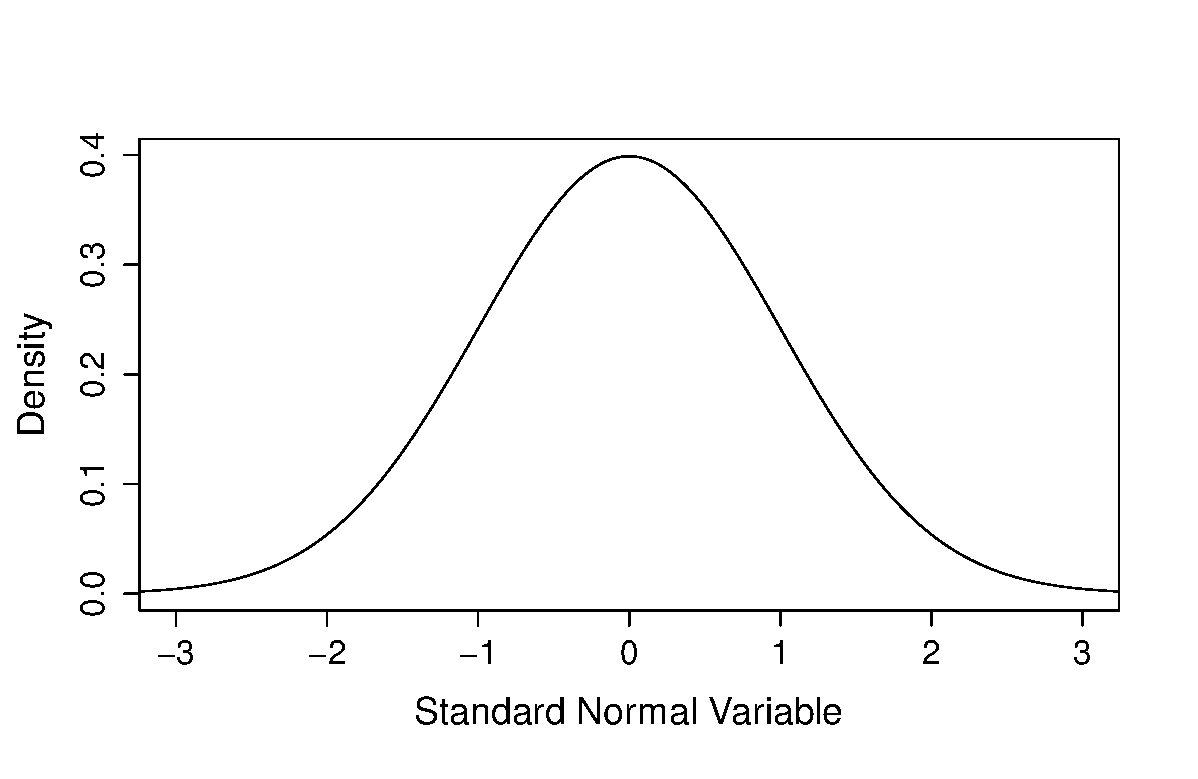
\includegraphics[width=0.95\textwidth, trim = 0.0cm 0.5cm 0.3cm 0.5cm, clip]{ZNormal}
\end{center}

\begin{itemize}
\item The letter $Z$ is used to denote standard normal variables: $Z \sim \text{Normal}(\mu=0,\sigma=1)$
\end{itemize}

\end{frame}


\subsection{Normal Tables}
\begin{frame}{\bf \tcb{Normal Tables}}

The normal tables show {\bf greater than} probabilities:\\[-0.1cm]
\begin{align*}
\boxed{\Pr(Z > z)}\\[-0.4cm]
\end{align*}
but only for positive values of $z$.\\[0.8cm]

We look up the $z$ value in the row/column headings and to find the relevant probability.\\[0.8cm]

{\bf Rows} show the \emph{first decimal place} of $z$ and the {\bf columns} show the \emph{second decimal place}.


\end{frame}



\subsection{Normal Tables Examples}
\begin{frame}{\bf \tcb{Normal Tables Examples}}

\begin{align*}
\bullet \quad \Pr(Z > 0.40) &= 0.3446 \qquad
&\bullet \quad\Pr(Z > 0.45) &= 0.3264\\[0.3cm]
\bullet \quad\Pr(Z > 1.08) &= 0.1401
&\bullet \quad\Pr(Z > 1.80) &= 0.0359\\[0.3cm]
\bullet \quad\Pr(Z > 2.00) &= 0.02275
&\bullet \quad\Pr(Z > 2.63) &= 0.00427\\[0.3cm]
\end{align*}

We calculate \emph{less than} probabilities using the \emph{complement} rule:
\begin{align*}
\bullet \quad \Pr(Z < 0.40) &= 1 - \Pr(Z > 0.40) = 1 - 0.3446 = 0.6554\\[0.3cm]
\bullet \quad \Pr(Z < 1.08) &= 1 - \Pr(Z > 1.08) = 1 - 0.1401 = 0.8599\\[0.3cm]
&\ldots \text{ etc.}
\end{align*}

\end{frame}



\subsection{Symmetry Rule}
\begin{frame}{\bf \tcb{Symmetry Rule}}

So we can calculate probabilities for positive $z$ values, but what about {\bf negative} values?\\[0.6cm]

We must apply the {\bf symmetry rule} for \emph{standard normal variables}:\\
\begin{align*}
\boxed{\Pr(Z < -z) = \Pr(Z > z)}
\end{align*}
or, similarly,\\[-0.5cm]
\begin{align*}
\boxed{\Pr(Z > -z) = \Pr(Z < z)}.\\
\end{align*}

$\Rightarrow$ {\bf Flip the inequality} symbol and {\bf change the sign} of the $z$ value.\\[0.4cm]

{\footnotesize(Note: this is \emph{not} a general rule of probability - it can only be used for the standard normal distribution)}

\end{frame}



\subsection{Symmetry Rule: Example 1}
\begin{frame}{\bf \tcb{Symmetry Rule: Example 1}}
\begin{adjustwidth}{-0.2cm}{}
\begin{tabular}{c@{}c@{}c}
$\Pr(Z < -1.5)$ &$=$& $\Pr(Z > 1.5)$ \\
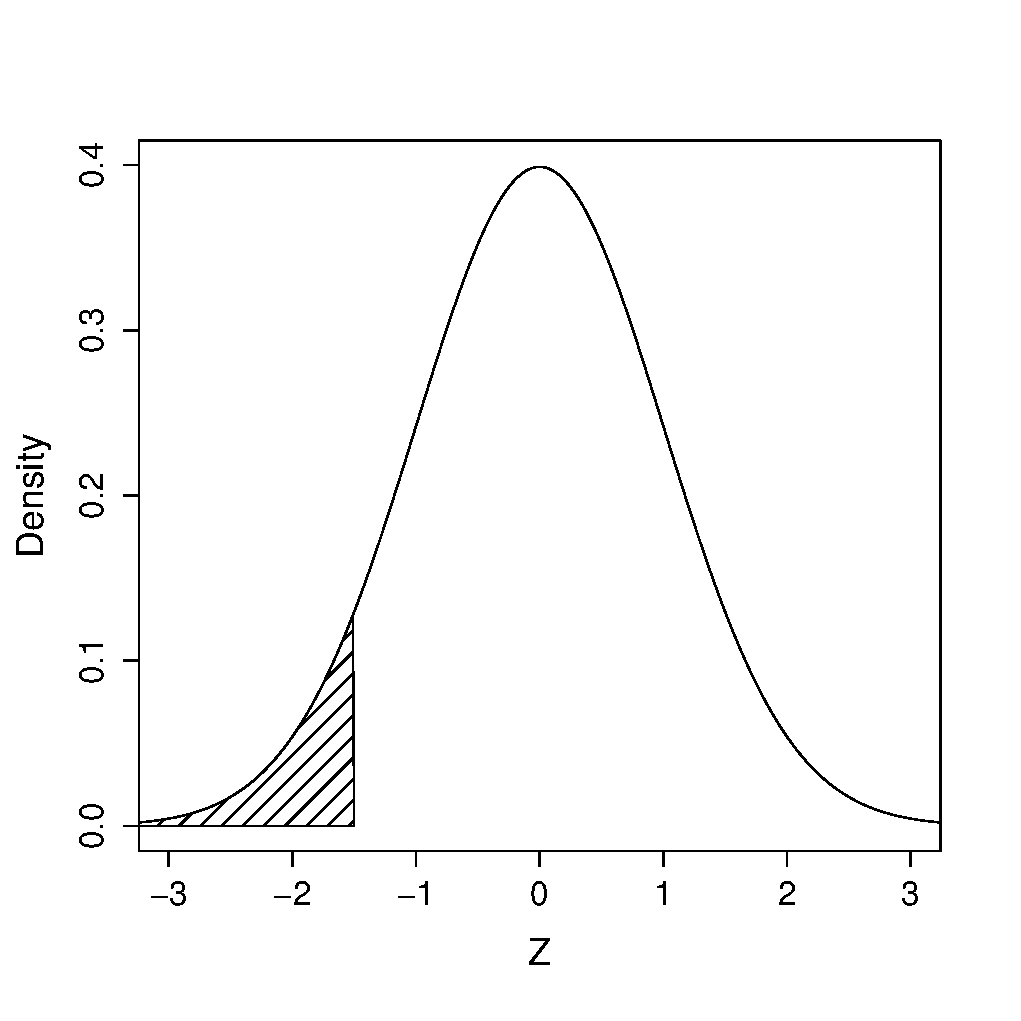
\includegraphics[width=0.5\textwidth, trim = 0.0cm 0.5cm 0.3cm 0.5cm, clip]{Symmetry1b}
&&
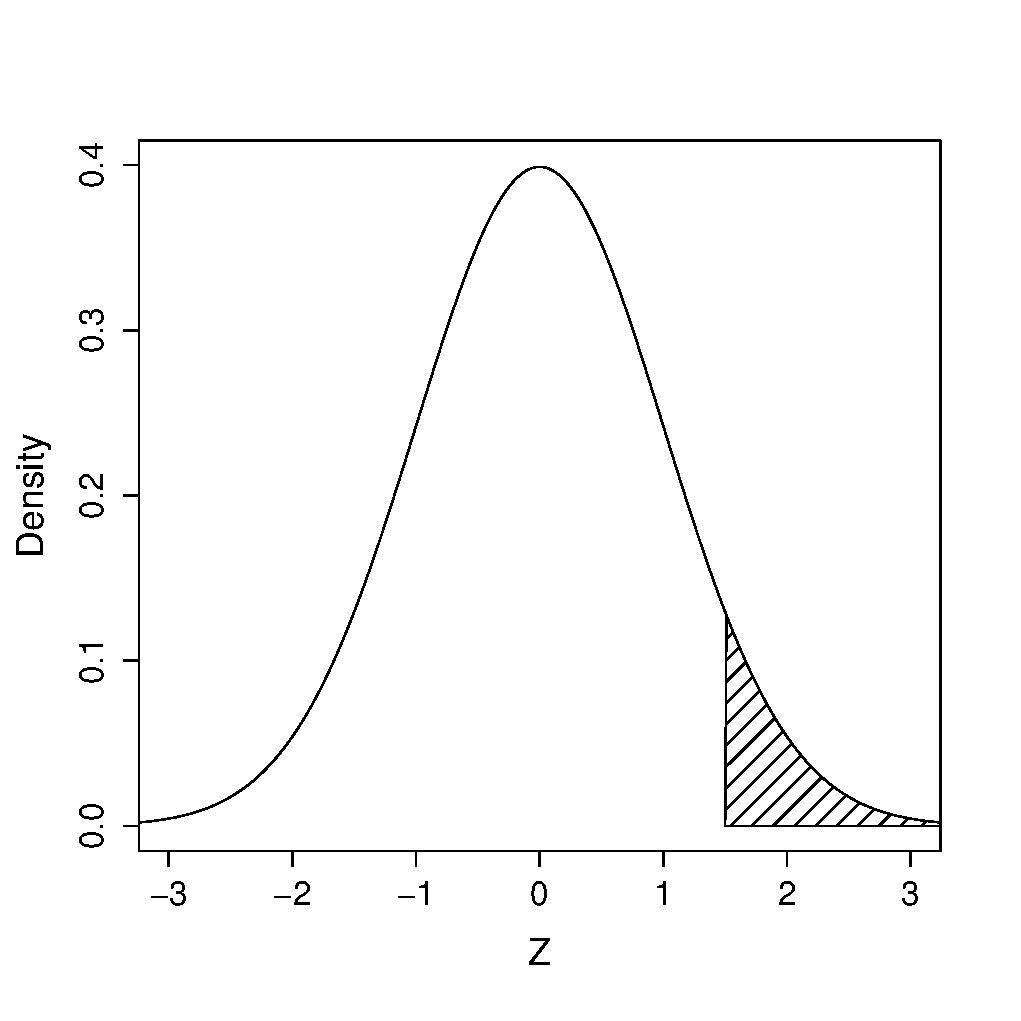
\includegraphics[width=0.5\textwidth, trim = 0.0cm 0.5cm 0.3cm 0.5cm, clip]{Symmetry1a}
\end{tabular}
\end{adjustwidth}

\end{frame}


\subsection{Symmetry Rule: Example 2}
\begin{frame}{\bf \tcb{Symmetry Rule: Example 2}}
\begin{adjustwidth}{-0.2cm}{}
\begin{tabular}{c@{}c@{}c}
$\Pr(Z > -1.5)$ &$=$& $\Pr(Z < 1.5)$ \\
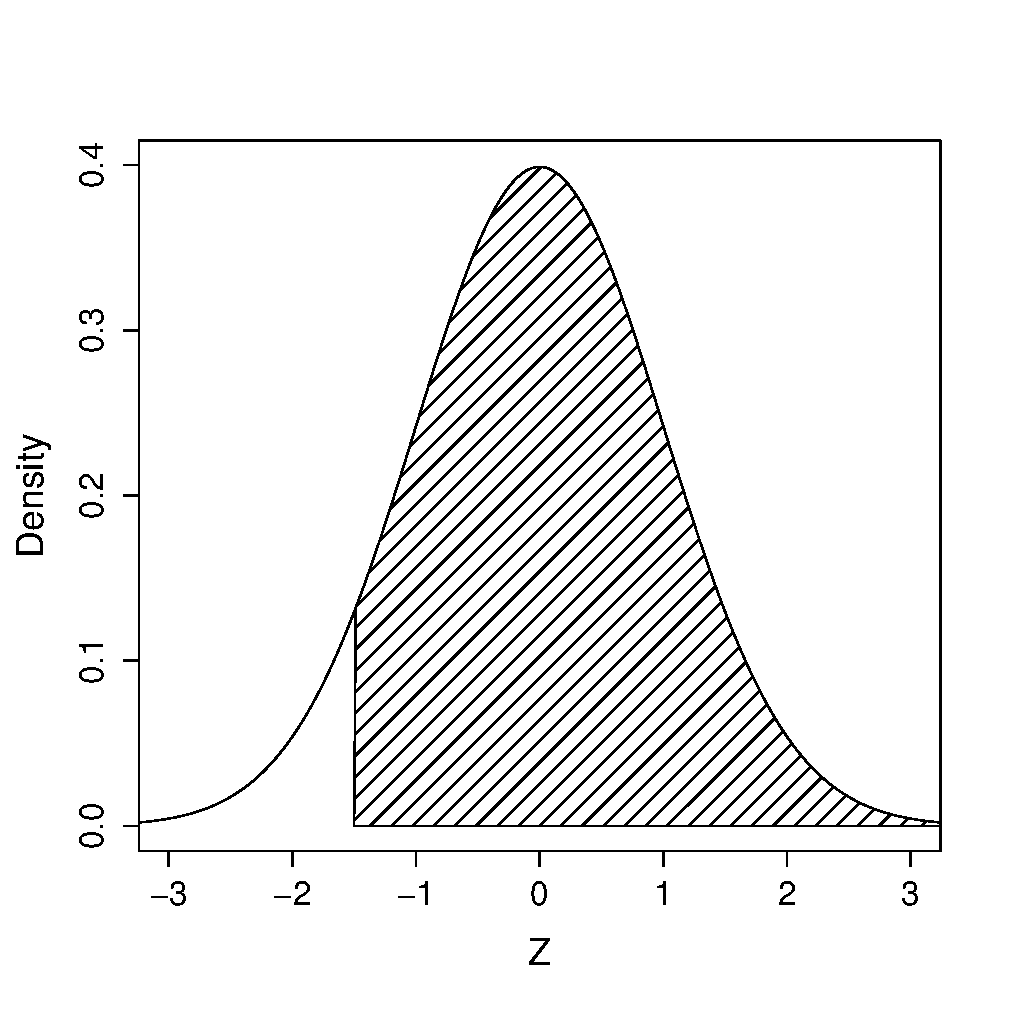
\includegraphics[width=0.5\textwidth, trim = 0.0cm 0.5cm 0.3cm 0.5cm, clip]{Symmetry2b}
&&
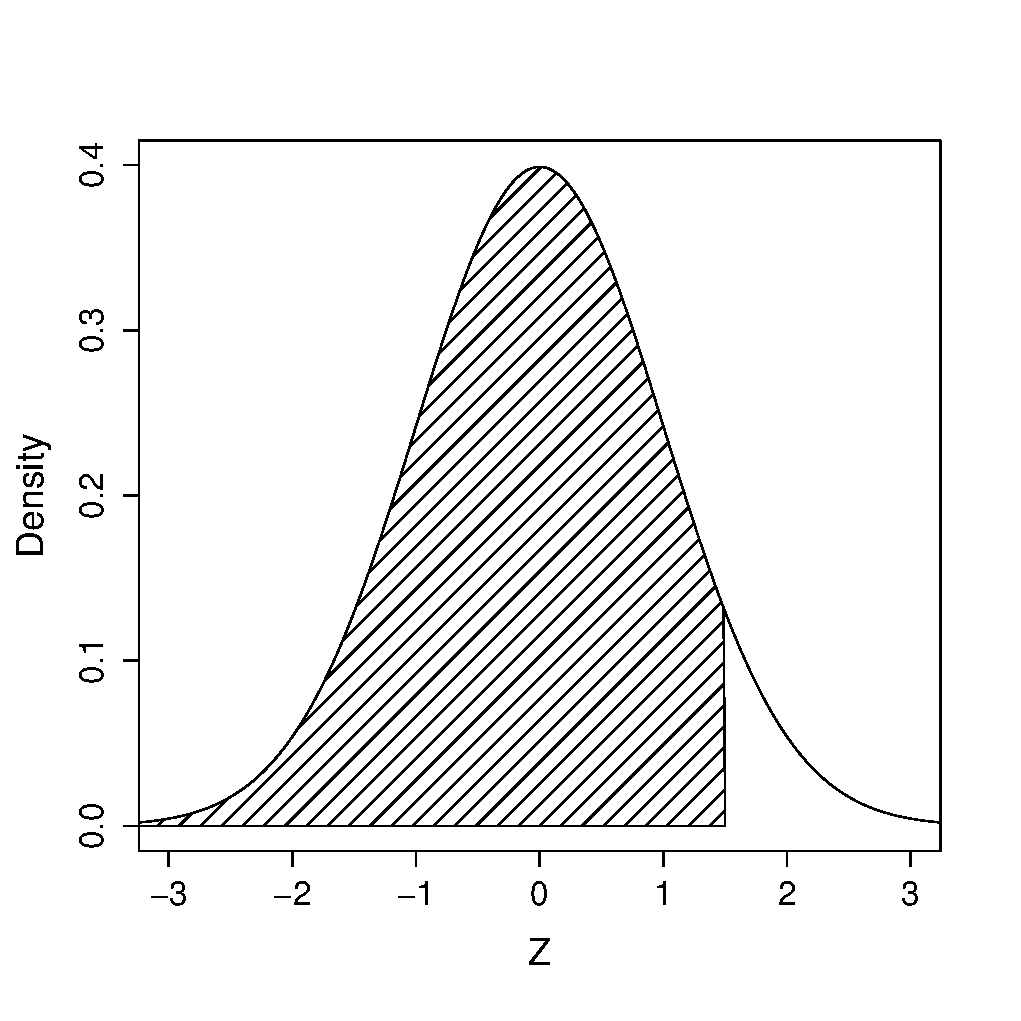
\includegraphics[width=0.5\textwidth, trim = 0.0cm 0.5cm 0.3cm 0.5cm, clip]{Symmetry2a}
\end{tabular}
\end{adjustwidth}


\end{frame}




\subsection{Normal Tables Examples}
\begin{frame}{\bf \tcb{Normal Tables Examples}}

\begin{align*}
\Pr(Z < -1.74) &= \Pr(Z > 1.74) \tag{symmetry rule} \\[0.2cm]
&= 0.0409. \tag{using tables} \\
\end{align*}

\begin{align*}
\Pr(Z > -0.60) &= \Pr(Z < 0.60) \tag{symmetry rule} \\[0.2cm]
&= 1 - \Pr(Z > 0.60) \tag{complement rule} \\[0.2cm]
&= 1 - 0.2743 = 0.7257. \tag{using tables} \\
\end{align*}


\end{frame}




\subsection{Normal Tables Examples}
\begin{frame}{\bf \tcb{Normal Tables Examples}}

\begin{align*}
\Pr(-1.00 < Z < 0.85) &= \Pr(Z > -1.00) - \Pr(Z > 0.85) \\[0.3cm]
&= \Pr(Z < 1.00) - \Pr(Z > 0.85) \\[0.3cm]
&= \left[1 - \Pr(Z > 1.00)\right] - \Pr(Z > 0.85) \\[0.3cm]
&= (1 - 0.1587) - 0.1977 \\[0.3cm]
&= 0.8403 - 0.1977 \\[0.3cm]
&= 0.6426.
\end{align*}

\end{frame}



\subsection{Question 1}
\begin{frame}{\bf \tcb{Question 1}}

Calculate the following:\\[0.3cm]
\begin{enumerate}[a)]\itemsep0.3cm
\item $\Pr(Z > 0.83)$.
\item $\Pr(Z < 1.05)$.
\item $\Pr(1 < Z < 2)$.
\item $\Pr(Z < -1.8)$.
\item $\Pr(-1 < Z < 1)$.
\item The value of $z$ such that $\Pr(Z > z) = 0.1$.
\end{enumerate}

\end{frame}




\section{Standardising}
\subsection{Standardising Normal Variables}
\begin{frame}{\bf \tcb{Standardising Normal Variables}}

For a normally distributed variable $X \sim \text{Normal}(\mu, \sigma)$, we can convert to a \emph{standard normal variable} via:\\
\begin{align*}
\boxed{Z = \frac{X-\mu}{\sigma}} \sim \text{Normal}(\mu=0, \sigma=1),\\[-0.3cm]
\end{align*}
i.e., we subtract the mean and divide by the standard deviation.\\[0.6cm]

This process is called {\bf standardising} and the resulting $Z$ value is typically referred to as a {\boldmath$Z$} {\bf score}.\\[0.6cm]

The $Z$ score is the \emph{number of standard deviations from the mean}.


\end{frame}



\subsection{Example: Salary}
\begin{frame}{\bf \tcb{Example: Salary}}
Earlier we had that $X \sim \text{Normal}(\mu=30,\sigma=4)$ and approximated probabilities (this is unsatisfactory).\\[0.6cm]

Now we can standardise the variable:\\
\begin{align*}
Z = \frac{X-\mu}{\sigma} = \frac{X-30}{4}\\[-0.2cm]
\end{align*}
and then use the normal tables to find the \emph{exact} probabilities.

\end{frame}


\subsection{Example: Salary}
\begin{frame}{\bf \tcb{Example: Salary}}
What is the probability that salary is greater than \texteuro{26}k?
\begin{align*}
\text{standardise: } Z &= \frac{26-30}{4} = \frac{-4}{4} = -1\\[0.4cm]
\Rightarrow \Pr(X > 26) &= \Pr(Z > -1)\\[0.1cm]
&= \Pr(Z < 1)\\[0.1cm]
&= 1 - \Pr(Z > 1)\\[0.1cm]
&= 1 - 0.1587\\[0.1cm]
&=  0.8413.\\[-0.2cm]
\end{align*}

Note that \texteuro{26}k is 1 standard deviation \emph{below} the mean $\Rightarrow$ $Z = -1$.

\end{frame}


\subsection{Example: Salary}
\begin{frame}{\bf \tcb{Example: Salary}}\label{normexampletab}

What is the probability that salary is between \texteuro{26}k and \texteuro{34}k?
\begin{align*}
\Pr(26 < X < 34) &= \Pr(X > 26) - \Pr(X > 34) \\[0.1cm]
&= 0.8413 - \Pr(Z > \tfrac{34-30}{4}) \\[0.1cm]
&= 0.8413 - \Pr(Z > 1) \\[0.1cm]
&= 0.8413 - 0.1587 \\[0.1cm]
&= 0.6826.\\
\end{align*}

What is the probability that salary is greater than \texteuro{36}k?
\begin{align*}
\Pr(X > 36) &= \Pr(Z > \tfrac{36-30}{4}) \\[0.1cm]
&= \Pr(Z > 1.5) \\[0.1cm]
&= 0.0668.
\end{align*}

\end{frame}




\subsection{Question 2}
\begin{frame}{\bf \tcb{Question 2}}

Assume that 12V batteries are produced in a factory. Due to slight variations, the actual voltage is $X \sim \text{Normal}(\mu=12,\sigma=0.1)$, i.e., not every battery is exactly 12V. Calculate the following:\\[0.3cm]

\begin{enumerate}[a)]\itemsep0.3cm
\item The proportion with more than 12.15V.
\item The proportion with less than 12.38V.
\item The proportion within the specification limits $12$V $\pm$ $0.15$V.
\item The value of $x$ such that $\Pr(X < x) = 0.9$.
\item The value of $x$ such that $\Pr(X < x) = 0.1$.
\end{enumerate}

\end{frame}




\subsection{R Code}
\begin{frame}{\bf \tcb{R Code}}
For the normal distribution we calculate \emph{greater than} probabilities, i.e., $\Pr(X > x)$.\\[0.4cm]

\begin{tabular}{|l|}
\hline
Examples: \\[0.2cm]
\texttt{pnorm(26,mean=30,sd=4,lower=F)} \\
gives \texttt{0.8413447}.\\[0.2cm]
\texttt{pnorm(34,mean=30,sd=4,lower=F)} \\
gives \texttt{0.1586553}.\\[0.2cm]
\texttt{pnorm(36,mean=30,sd=4,lower=F)} \\
gives \texttt{0.0668072}.\\[0.2cm]
\hline
\multicolumn{1}{c}{}\\[0.0cm]
\end{tabular}

Compare this with slide \pageref{normexampletab}.\\[0.6cm]

\end{frame}




\subsection{R Code}
\begin{frame}{\bf \tcb{R Code}}
We can \emph{generate} normal random variables as follows:\\[0.5cm]

\begin{tabular}{|l|}
\hline
Example: \\[0.2cm]
\texttt{rnorm(100,mean=30,sd=4)} \\
generates 100 Normal$(\mu=30,\sigma=4)$ variables.\\
\hline
\multicolumn{1}{c}{}\\[0.2cm]
\end{tabular}


\end{frame}



\section{Checking Normality}
\subsection{Checking Normality}
\begin{frame}{\bf \tcb{Checking Normality}}

For a given set of data, it is often useful to check if the distribution looks approximately normal.\\[0.8cm]

If this does turn out to be the case, we can calculate probabilities as shown on the previous slides.\\[0.8cm]

We can also apply the \emph{t test} to small samples that are approximately normal (more on this later).

\end{frame}



\subsection{Histogram / Boxplot}
\begin{frame}{\bf \tcb{Histogram / Boxplot}}\label{histbox}
\begin{adjustwidth}{-0.2cm}{}
\begin{tabular}{c@{}c@{}c}
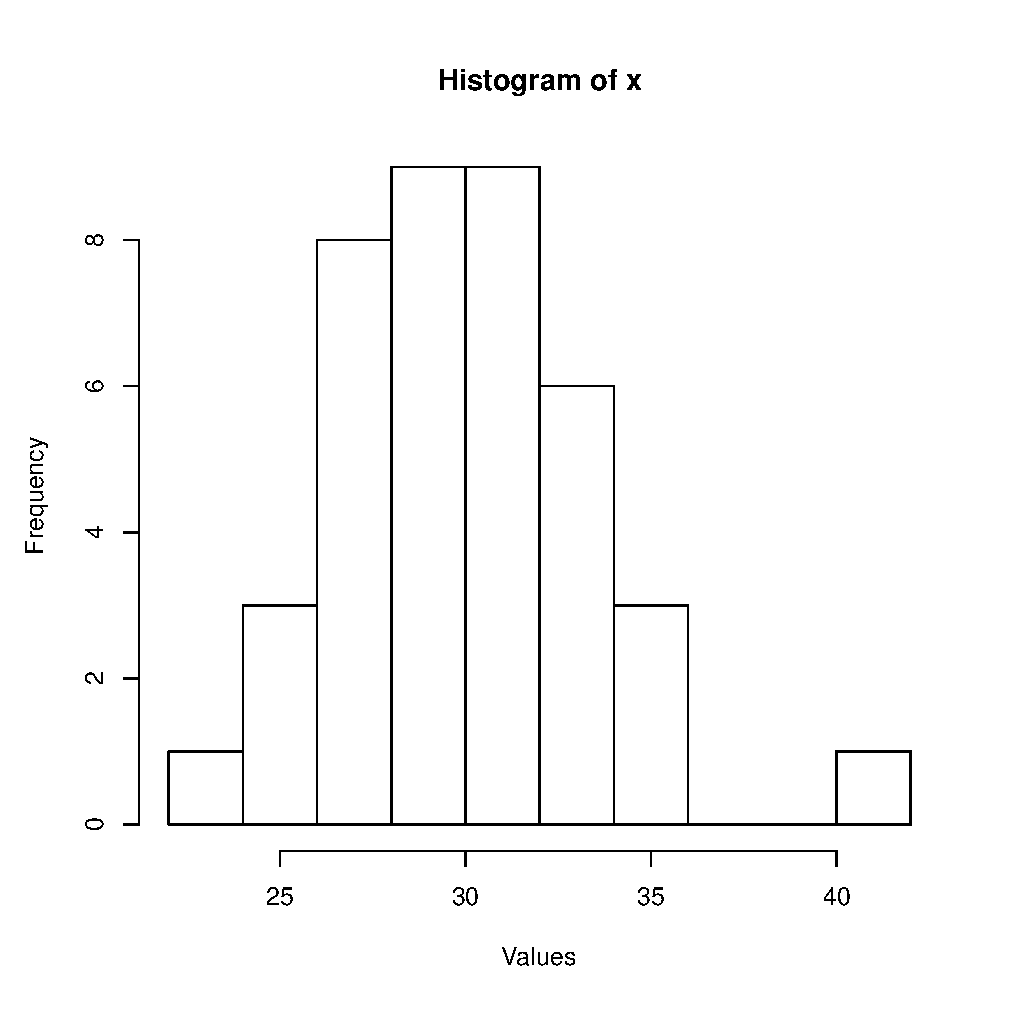
\includegraphics[width=0.5\textwidth, trim = 0.0cm 0.5cm 0.3cm 0.5cm, clip]{HistNorm}
&&
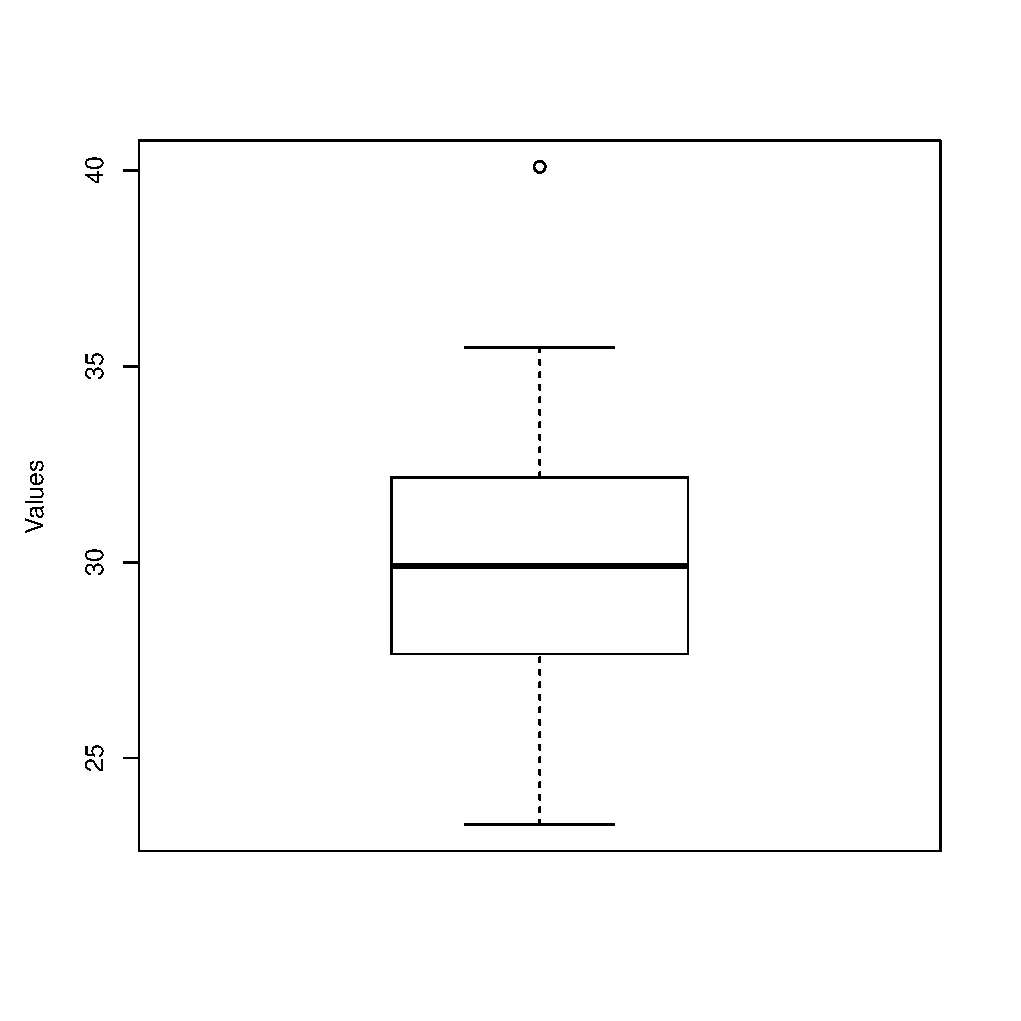
\includegraphics[width=0.5\textwidth, trim = 0.0cm 0.5cm 0.3cm 0.5cm, clip]{BoxplotNorm}
\end{tabular}
\end{adjustwidth}

Together, the histogram and boxplot can tell us about the distribution of values. We see that the above looks approximately normal.

\end{frame}


\subsection{Q-Q Plot}
\begin{frame}{\bf \tcb{Q-Q Plot}}
A more useful check for normality is the {\bf quantile-quantile plot}.\\[0.8cm]

The Q-Q plot compares the \emph{quantiles} of the sample of data to those of a theoretical normal distribution.\\[0.8cm]

If the data is approximately normally distributed, the quantiles match and the Q-Q points lie on a straight line.\\[0.8cm]

Note: a quantile is a more general concept than \emph{quartiles} which we studied earlier. In fact quartiles are the 4-quantiles.\\
{\footnotesize(For your information: the 100-quantiles are known as percentiles)}

\end{frame}

\subsection{Q-Q Plot}
\begin{frame}{\bf \tcb{Q-Q Plot}\\[-1.1cm]}
\begin{center}
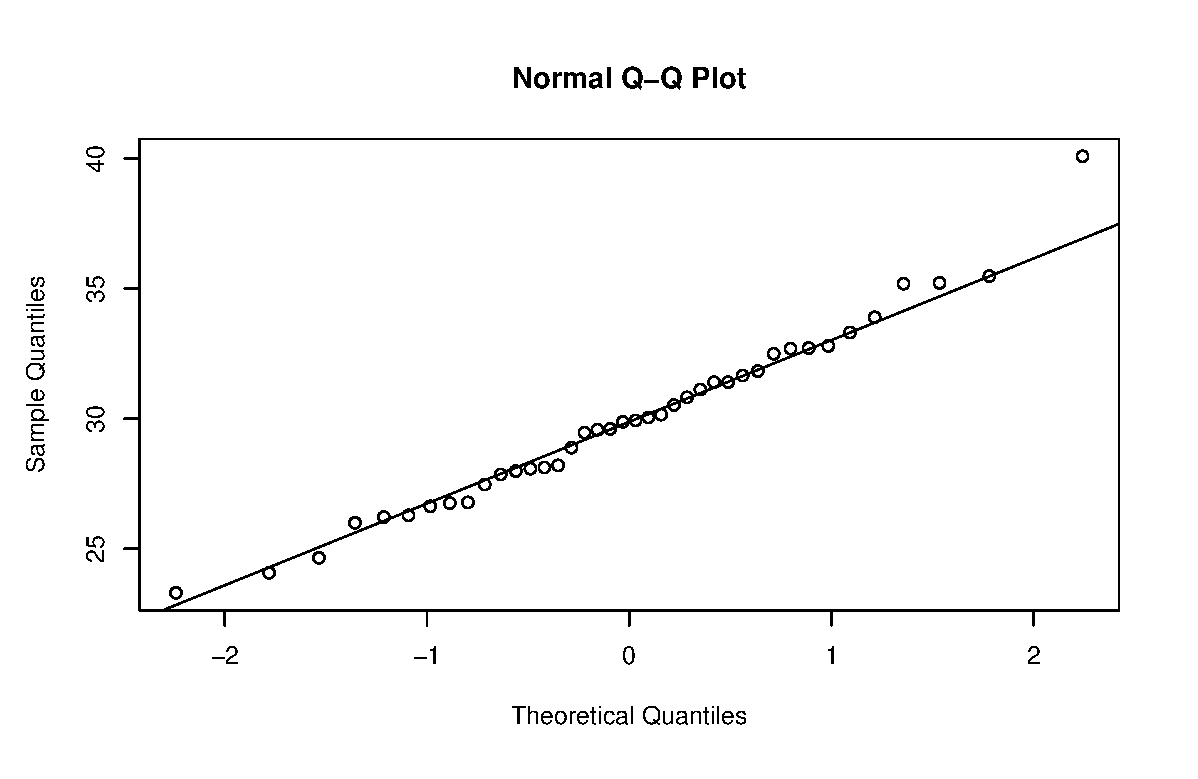
\includegraphics[width=0.87\textwidth, trim = 0.0cm 0.5cm 0.3cm 0.5cm, clip]{QQNorm}
\end{center}
\begin{itemize}
\item The data appears to be approximately normally distributed apart from one outlier {\footnotesize(compare with the histogram and boxplot on slide \pageref{histbox})}.
\end{itemize}

\end{frame}


\subsection{R Code}
\begin{frame}{\bf \tcb{R Code}}
The graphs on the previous slides can be produced via:\\[0.5cm]

\begin{tabular}{|l|}
\hline
\texttt{set.seed(112187721)} \\
\texttt{x = round(rnorm(40, mean=30, sd=4),3)} \\
\texttt{hist(x, xlab="Values")} \\
\texttt{boxplot(x, ylab="Values")} \\
\texttt{qqnorm(x); qqline(x)} \\
\hline
\multicolumn{1}{c}{}\\[0.2cm]
\end{tabular}

A sample of 40 Normal$(\mu=30,\sigma=4)$ variables were generated - try with different sample sizes.\\[0.3cm]

Note the use of \texttt{set.seed} so that you can reproduce the exact data used in these slides - try the above without \texttt{set.seed}.

\end{frame}





\subsection{R Code}
\begin{frame}{\bf \tcb{R Code}}
See what happens when we generate from an exponential distribution:\\[0.5cm]


\begin{tabular}{|l|}
\hline
\texttt{set.seed(112187721)} \\
\texttt{x = round(rexp(40, rate=1),3)} \\
\texttt{hist(x, xlab="Values")} \\
\texttt{boxplot(x, ylab="Values")} \\
\texttt{qqnorm(x); qqline(x)} \\
\hline
\multicolumn{1}{c}{}\\[0.2cm]
\end{tabular}

The output of the above code is shown on the next two slides. We can see that this data is not normally distributed.

\end{frame}



\subsection{Histogram / Boxplot}
\begin{frame}{\bf \tcb{Histogram / Boxplot}}
\begin{adjustwidth}{-0.2cm}{}
\begin{tabular}{c@{}c@{}c}
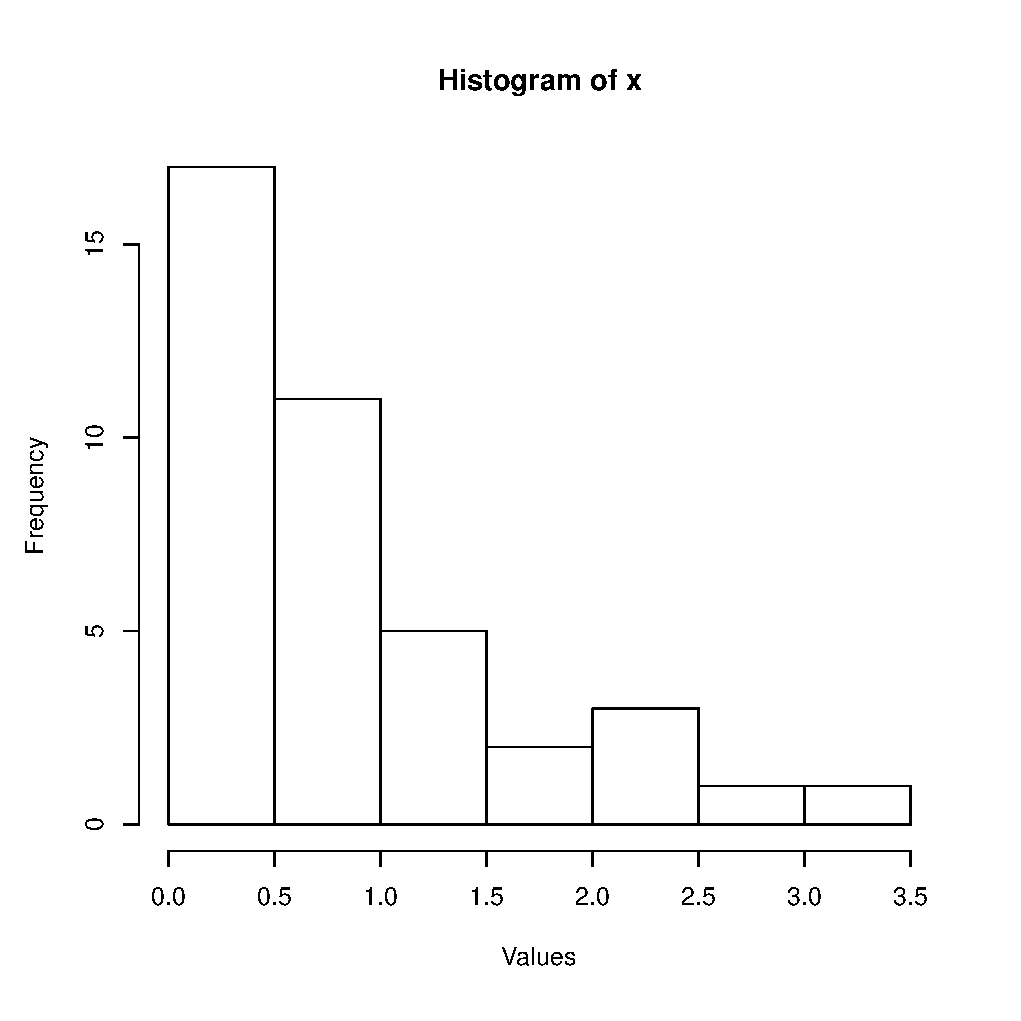
\includegraphics[width=0.5\textwidth, trim = 0.0cm 0.5cm 0.3cm 0.5cm, clip]{HistExp}
&&
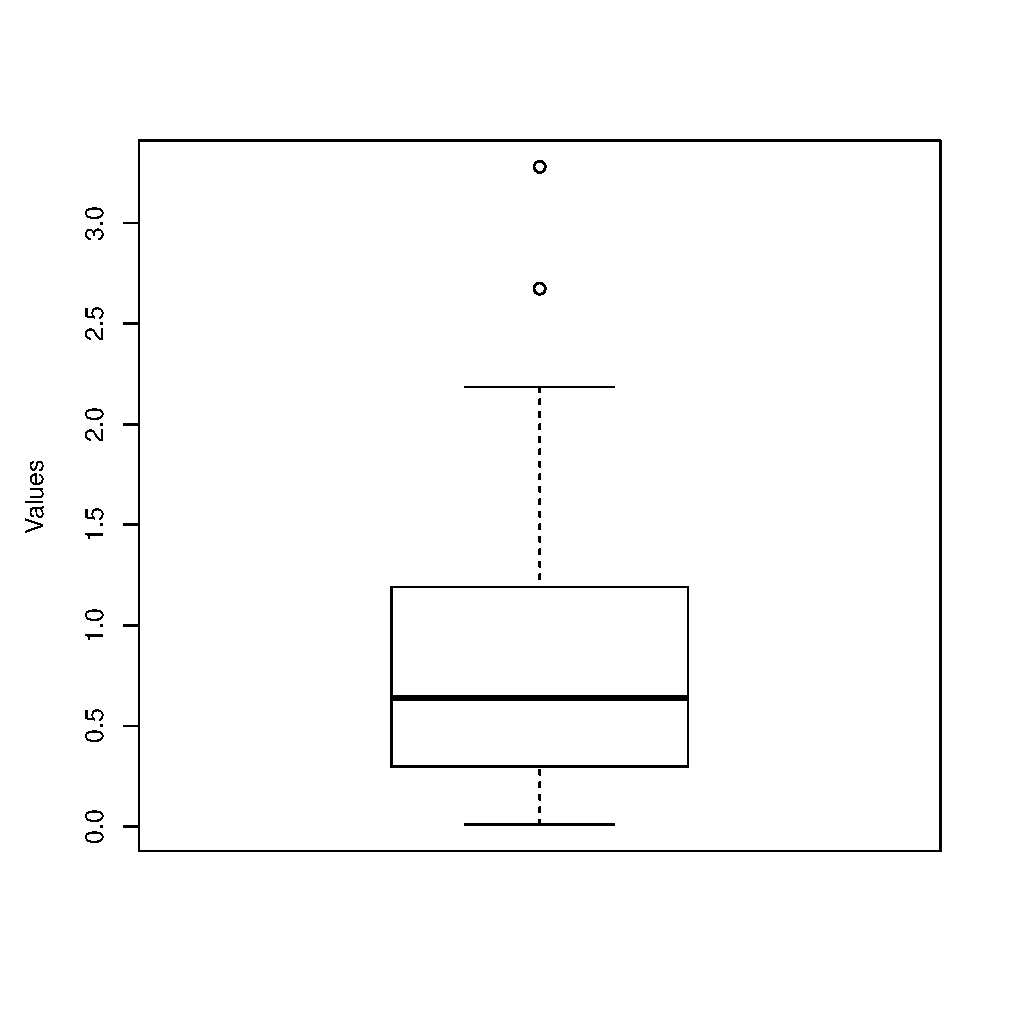
\includegraphics[width=0.5\textwidth, trim = 0.0cm 0.5cm 0.3cm 0.5cm, clip]{BoxplotExp}
\end{tabular}
\end{adjustwidth}

\end{frame}


\subsection{Q-Q Plot}
\begin{frame}{\bf \tcb{Q-Q Plot}\\[-1.1cm]}
\begin{center}
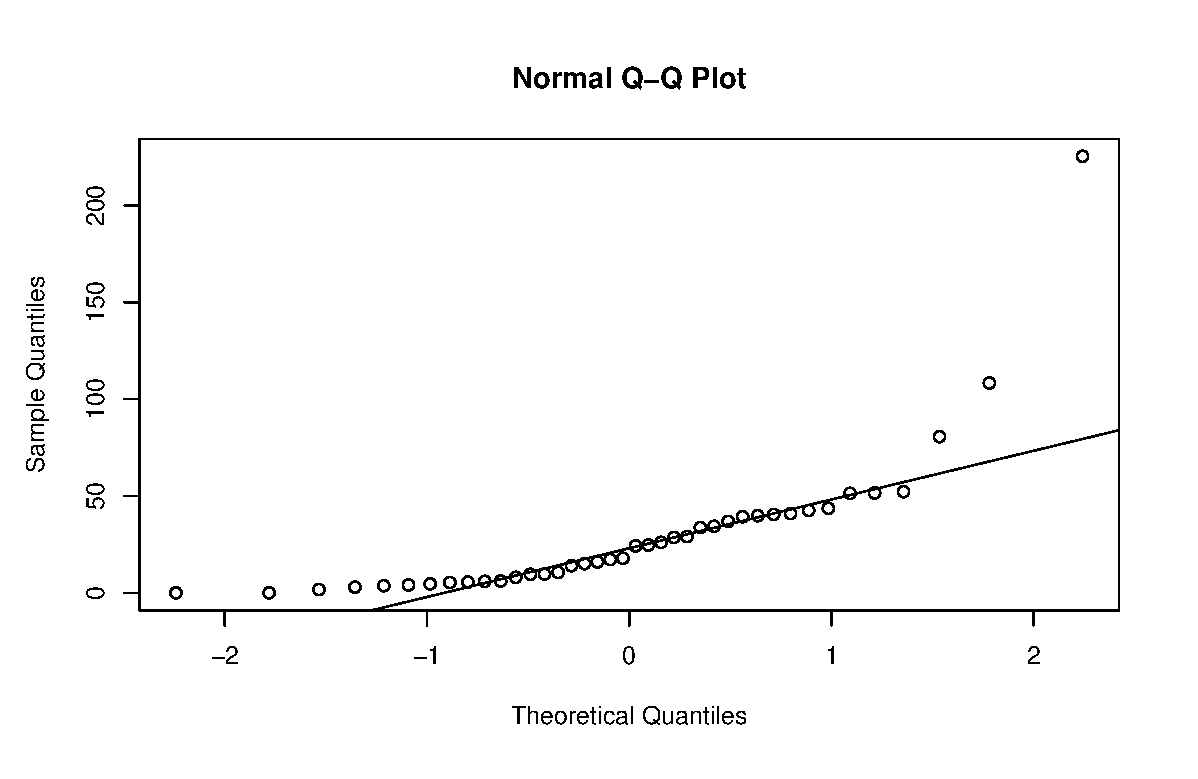
\includegraphics[width=0.87\textwidth, trim = 0.0cm 0.5cm 0.3cm 0.5cm, clip]{QQExp}
\end{center}

\end{frame}









\end{document} 